%%%%%%%%%%%%%%%%%%%%%%%%%%%%%%%%%%%%%%%%%
% NIWeek 2014 Poster by T. Reveyrand
% www.microwave.fr
% http://www.microwave.fr/LaTeX.html
% ---------------------------------------
%
% Original template created by:
% Brian Amberg (baposter@brian-amberg.de)
%
% This template has been downloaded from:
% http://www.LaTeXTemplates.com
%
% License:
% CC BY-NC-SA 3.0 (http://creativecommons.org/licenses/by-nc-sa/3.0/)
%
%%%%%%%%%%%%%%%%%%%%%%%%%%%%%%%%%%%%%%%%%

%----------------------------------------------------------------------------------------
%   PACKAGES AND OTHER DOCUMENT CONFIGURATIONS
%----------------------------------------------------------------------------------------

\documentclass[a0paper,portrait]{baposter}

\usepackage[font=small,labelfont=bf]{caption} % Required for specifying captions to tables and figures
\usepackage{booktabs} % Horizontal rules in tables
\usepackage{relsize} % Used for making text smaller in some places
\usepackage{amsmath,amsfonts,amssymb,amsthm} % Math packages
\usepackage{eqparbox}
\usepackage{textcomp}
\usepackage{caption}
\usepackage{subcaption}
\usepackage{graphicx}
\usepackage{listings}
\usepackage{enumitem}
\usepackage{pgf}
\usepackage{tikz}
\usetikzlibrary{positioning}
\usepackage[utf8]{inputenc}
\usetikzlibrary{arrows,automata}
\usetikzlibrary{positioning}


\graphicspath{{figures/}} % Directory in which figures are stored

 \definecolor{bordercol}{RGB}{40,40,40} % Border color of content boxes
 \definecolor{headercol1}{RGB}{186,215,230} % Background color for the header in the content boxes (left side)
 \definecolor{headercol2}{RGB}{120,120,120} % Background color for the header in the content boxes (right side)
 \definecolor{headerfontcol}{RGB}{0,0,0} % Text color for the header text in the content boxes
 \definecolor{boxcolor}{RGB}{210,235,250} % Background color for the content in the content boxes


\tikzset{
    state/.style={
           rectangle,
           rounded corners,
           draw=black, very thick,
           minimum height=2em,
           inner sep=2pt,
           text centered,
           },
}

\begin{document}

\setlength{\fboxsep}{0pt}

\background{ % Set the background to an image (background.pdf)
\begin{tikzpicture}[remember picture,overlay]
\draw (current page.north west)+(-2em,2em) node[anchor=north west]
{
\includegraphics[height=1.1\textheight]{background}};
\end{tikzpicture}
}

\begin{poster}{
grid=false,
columns=4,
borderColor=bordercol, % Border color of content boxes
headerColorOne=headercol1, % Background color for the header in the content boxes (left side)
headerColorTwo=headercol2, % Background color for the header in the content boxes (right side)
headerFontColor=headerfontcol, % Text color for the header text in the content boxes
boxColorOne=boxcolor, % Background color for the content in the content boxes
headershape=roundedright, % Specify the rounded corner in the content box headers
headerfont=\Large\sf\bf, % Font modifiers for the text in the content box headers
textborder=rectangle,
background=none,
headerborder=open, % Change to closed for a line under the content box headers
boxshade=plain
}
{
\includegraphics[width=3cm]{BiATA2019.png}}
%
%----------------------------------------------------------------------------------------
%   TITLE AND AUTHOR NAME
%----------------------------------------------------------------------------------------
%
{ \bf  \huge {Improved Architecture of Artificial Neural Network for Secondary Structure Analysis} }  % Poster title
{\vspace{0.3em} \smaller \textbf{Polina Lunina$^1$}, Semyon Grigorev$^1$ \\  % Author names
\smaller \it $^1${Saint Petersburg State University, JetBrains Reserach, St. Petersburg, Russia } \\ % Author email addresses
\smaller  {\textbf{E-mail:} lunina\_polina@mail.ru, semyon.grigorev@jetbrains.com}}
{
\includegraphics[width=3cm]{SPbGU_Logo.png}} % University/lab logo


%----------------------------------------------------------------------------------------
%   INTRODUCTION
%----------------------------------------------------------------------------------------
\headerbox {Motivation}{name=introduction,column=0,row=0, span=2}{

An approach for biological sequences processing by combination of formal grammars and neural networks is proposed in the work~\cite{grigorevcomposition}.
While classical way is to model secondary structure of the full sequence by using grammar, the proposed approach utilizes it only for primitive secondary structure features description. These features can be extracted by parsing algorithm and processed by using artificial neural network. It is shown that this approach is applicable for real-world data processing and some questions are formulated for future research. In this work we provide answers to some of them.  
}


\headerbox {Questions}{name=questions, column=2, row=0, span=2}{

\textbf{Is it possible to use convolutional neural networks for parsing result processing?} The result of parsing algorithm is a set of upper triangular boolean matrices. The original idea is to vectorize these matrices row by row and use DNNs for these vectors processing. Matrices can be also treated as bitmaps, where the false bits of matrix correspond to white pixels and the true bits to black ones. To handle these images we use network with a small number of convolutional layers followed by linearization and then the same structure as for vectorized data (dense and dropout layers with batch normalization).

\textbf{Is it possible to move parsing to network training step?} Parsing is the most time-consuming operation of the proposed solution. We solve this problem by using two-staged learning. At the first step, we prepare a neural network (vector- or image-based) for our task which takes parsed data as an input. After that we extend trained network with a number of input layers that should convert the original nucleotide sequence into parsing result. This way we create a network which can handle sequences, not parsing result. So, parsing is required only for training the base network.
}


\headerbox {Results}{name=results, column=0, row=0, span=2, below=introduction}{
We use the proposed improvements for tRNA sequences analysis tasks: classification of tRNA into 2 classes: eukaryotes and prokaryotes (EP) and 4 classes: archaea, bacteria, plants and fungi (ABFP). We use sequences from databases~\cite{trnadb1, trnadb2}. Results for both image- and vector-based classifiers are presented in the table, where base model means network which handles parsing result and extended model handles sequences and is based on the corresponding base model.
\begin{center}
\small
\begin{tabular}{|l||l|l||l|l|}
\hline
Classifier                                                               & \multicolumn{2}{l||}{EP}               & \multicolumn{2}{l|}{ABFP}           \\ \hline \hline
Approach   & Vectors  & Images   & Vectors      & Images     \\ \hline
\begin{tabular}[c]{@{}l@{}}Base model\\ accuracy\end{tabular}            & 94.1\%             & 96.2\%           & 86.7\%            & 93.3\%          \\ \hline
\begin{tabular}[c]{@{}l@{}}Extended model \\ accuracy\end{tabular}       & 97.5\%             & 97.8\%           & 96.2\%            & 95.7\%          \\ \hline
\begin{tabular}[c]{@{}l@{}}Total samples\\ (train:valid:test)\end{tabular} & \multicolumn{2}{l||}{20000:5000:10000} & \multicolumn{2}{l|}{8000:1000:3000} \\ \hline
\end{tabular}
\end{center}
}


\headerbox{Solution Overview}{name=solution,span=4,column=0,row=1,below=results}{

\begin{tikzpicture}[->,>=stealth']

\node[state,
      align = left,
      text width = 5cm](parser)
{
\textbf{Parser}\\
Parser extracts secondary structure features described by grammar. We use a matrix-based parsing algorithm~\cite{gsv}.
};


\node[state,
      right of=parser,
      node distance=6cm,
      align = left,
      text width = 5cm] (mtrx)
{
  \textbf{Matrices}\\
Parsing result for sequence $w$ and nonterminal $N$ is an upper-triangular boolean matrix $M_N$, where $M_N [i,j] = 1$, iff $w[i,j-1]$ is derivable from $N$.
};

\node[state,
      right of=mtrx,
      node distance=7.5cm,
      align = left,
      text width = 8cm](vector)
{
\textbf{Vectors}\\
We drop out the bottom left triangle
and vectorize the rest of matrix row by row. It requires the equal length of the input sequences, therefore we propose to either cut sequences or add some empty symbol till the definite length.
};

\node[state,
      below of=vector,
      node distance=3cm,
      align = left,
      text width = 8cm](image)
{
\textbf{Images}\\
We represent the false bits of matrix as white pixels and the true bits as black ones to get a bitmap image. This approach makes it possible to process sequences with different lengths since the images may be easily transformed to the same size.
};

\node[state,
      below of=parser,
      node distance=5.8cm,
      align = left,
      text width = 9.5cm](NN)
{
\textbf{Neural Networks}\\
 \vspace{0.2cm}
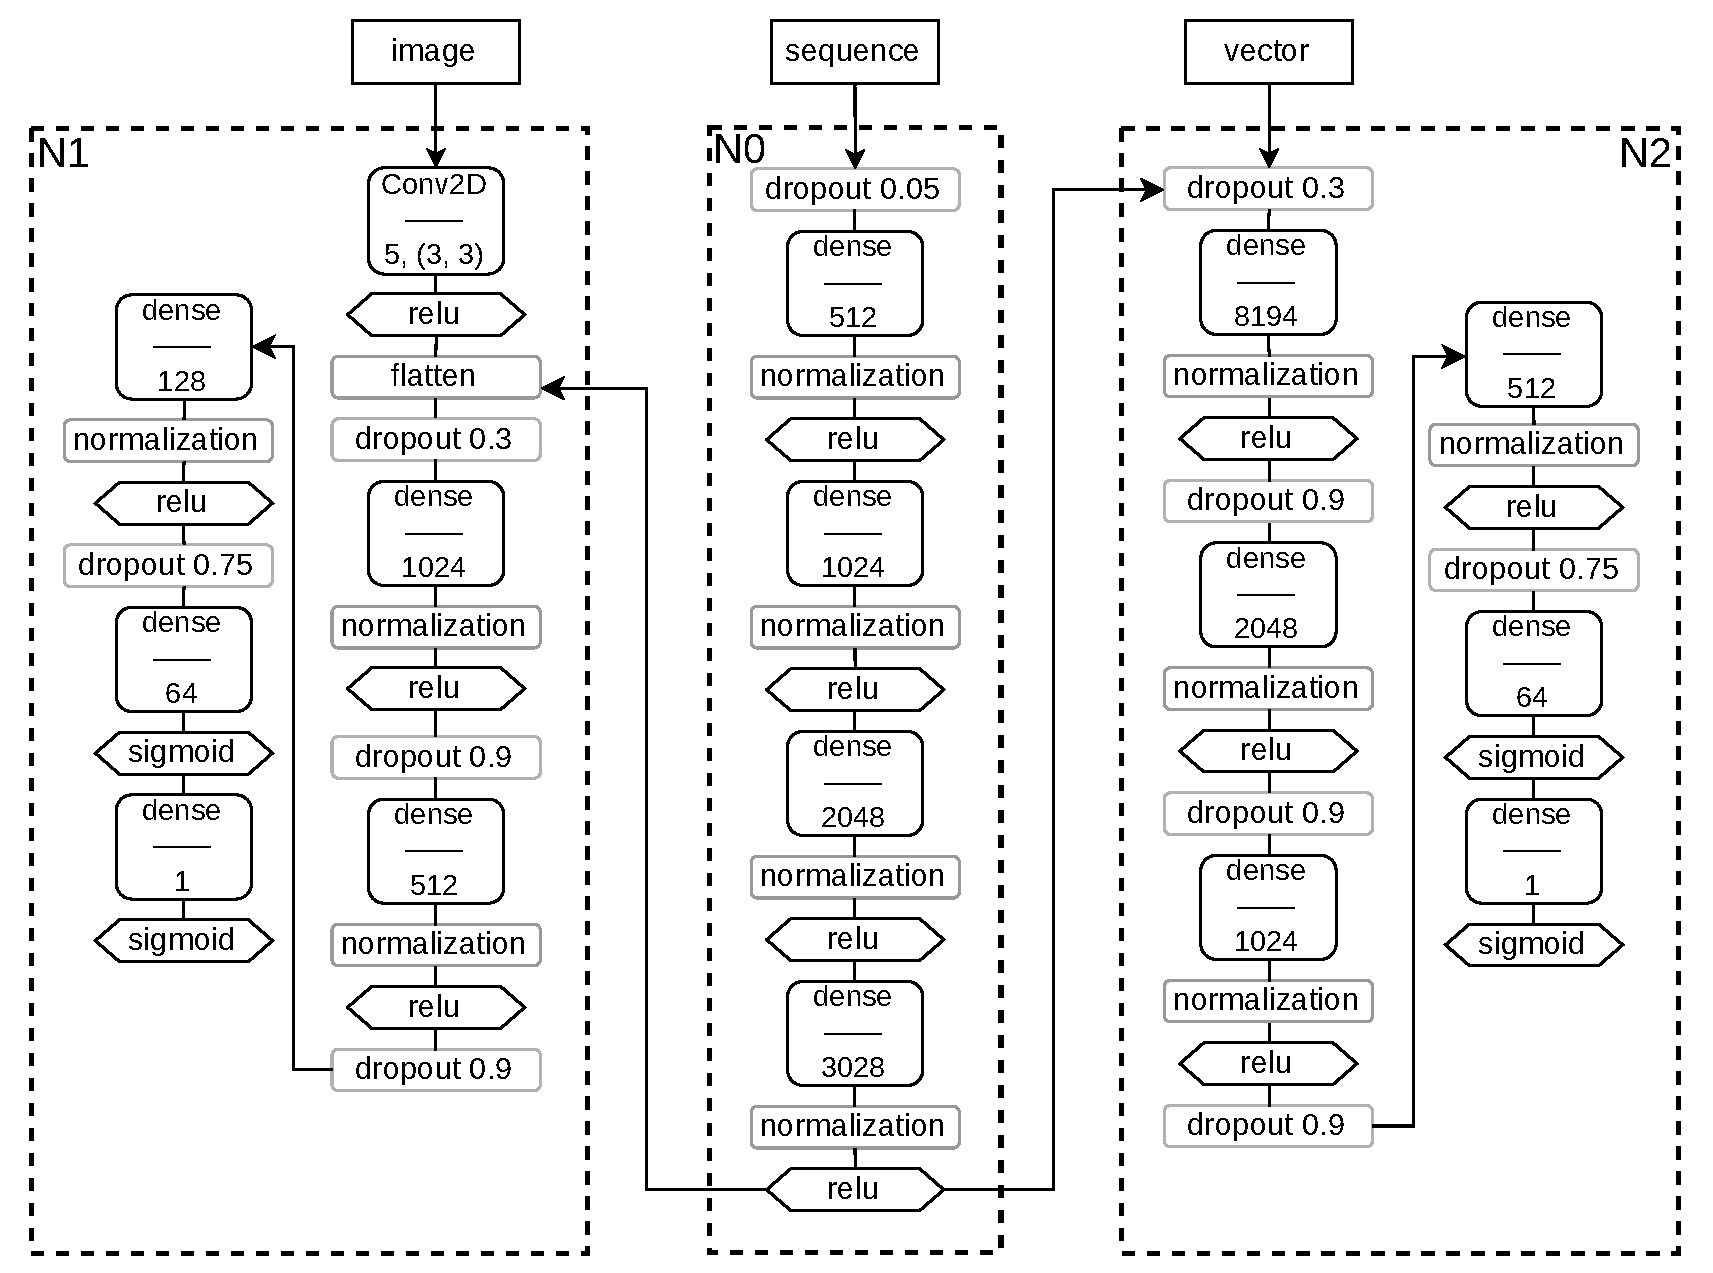
\includegraphics[width=9.5cm]{figures/nn_arch.pdf}

};

\node[state,
      above left=2cm and -1.5cm of NN,
      align=left,
      text width = 2cm] (grm)
 {
  \textbf{Grammar}
 };

\node[state,
      below of=grm,
      node distance=1cm,
      align = left,
      text width = 2cm] (sqs)
 {
 \textbf{Sequences}
 };

\node[state,
      below right=4cm and 3cm of parser,
      align = left,
      text width = 6cm](NN_info)
{
\textbf{Neural Networks}\\
\textbf{\texttt{N1}} is a model for images classification, \textbf{\texttt{N2}} is a model that classifies vectorized data and \textbf{\texttt{N0}} is the extension block which converts the original nucleotide sequence into a set of features which can be handled by using weights of \textbf{\texttt{N1}} or \textbf{\texttt{N2}}.


};

\path (grm.east) edge (parser.171)
 (sqs.east) edge (parser.193)
 (parser) edge (mtrx)
 (mtrx) edge (vector)
 (mtrx) edge [bend right] (image.west)
 (NN.-11) edge [-,dashed,] (NN_info)
 ;

\end{tikzpicture}
}


\headerbox {Future Research}
{name=app1,column=2,span=2, below=questions}
{
\begin{itemize}
\item Chimeric sequences filtration
\item Secondary structure prediction
\item Proteins functions prediction
\end{itemize}
}

%----------------------------------------------------------------------------------------
%   REFERENCES
%----------------------------------------------------------------------------------------

\headerbox {References}
{name=app2,column=2,span=2, below=solution}
{
\smaller % Reduce the font size in this block
\renewcommand{\section}[2]{\vskip 0.05em} % Get rid of the default "References" section title
%\nocite{*} % Insert publications even if they are not cited in the poster

\bibliographystyle{unsrt}
%\bibliographystyle{IEEEtran}
\bibliography{biblio} % Use biblio.bib as the bibliography file
}


\headerbox {Acknowledgments}{name=ack,column=0,span=2,below=solution}{
The research was supported by the Russian Science Foundation grant 

18-11-00100 and a grant from JetBrains Research.
}

\headerbox {Information}{name=info,column=0,span=2,below=ack}{
All materials are available on GitHub:

https://github.com/LuninaPolina/SecondaryStructureAnalyzer
}

\end{poster}

\end{document}
